\documentclass[8pt,aspectratio=169]{beamer}
\usetheme{Madrid}
\usepackage{graphicx}
\usepackage{booktabs}
\usepackage{adjustbox}
\usepackage{multicol}
\usepackage{amsmath}
\usepackage{amssymb}
\usepackage{tikz}
\usetikzlibrary{arrows.meta,positioning,shapes.callouts,shapes.geometric,decorations.pathreplacing}
\usepackage{hyperref}
\usepackage{algorithm}
\usepackage{algorithmic}

% Color definitions
\definecolor{mlblue}{RGB}{0,102,204}
\definecolor{mlpurple}{RGB}{51,51,178}
\definecolor{mllavender}{RGB}{173,173,224}
\definecolor{mllavender2}{RGB}{193,193,232}
\definecolor{mllavender3}{RGB}{204,204,235}
\definecolor{mllavender4}{RGB}{214,214,239}
\definecolor{mlorange}{RGB}{255, 127, 14}
\definecolor{mlgreen}{RGB}{44, 160, 44}
\definecolor{mlred}{RGB}{214, 39, 40}
\definecolor{mlgray}{RGB}{127, 127, 127}

% Additional colors for template compatibility
\definecolor{lightgray}{RGB}{240, 240, 240}
\definecolor{midgray}{RGB}{180, 180, 180}

% Backward compatibility: uppercase color names
\colorlet{MLPurple}{mlpurple}
\colorlet{MLBlue}{mlblue}
\colorlet{MLOrange}{mlorange}
\colorlet{MLGreen}{mlgreen}
\colorlet{MLRed}{mlred}
\colorlet{MLLavender}{mllavender}
\colorlet{MLGray}{mlgray}

% Apply custom colors to Madrid theme
\setbeamercolor{palette primary}{bg=mllavender3,fg=mlpurple}
\setbeamercolor{palette secondary}{bg=mllavender2,fg=mlpurple}
\setbeamercolor{palette tertiary}{bg=mllavender,fg=white}
\setbeamercolor{palette quaternary}{bg=mlpurple,fg=white}

\setbeamercolor{structure}{fg=mlpurple}
\setbeamercolor{section in toc}{fg=mlpurple}
\setbeamercolor{subsection in toc}{fg=mlblue}
\setbeamercolor{title}{fg=mlpurple}
\setbeamercolor{frametitle}{fg=mlpurple,bg=mllavender3}
\setbeamercolor{block title}{bg=mllavender2,fg=mlpurple}
\setbeamercolor{block body}{bg=mllavender4,fg=black}

% Remove navigation symbols
\setbeamertemplate{navigation symbols}{}

% Clean itemize/enumerate
\setbeamertemplate{itemize items}[circle]
\setbeamertemplate{enumerate items}[default]

% Reduce margins for more content space
\setbeamersize{text margin left=5mm,text margin right=5mm}

% Custom course footer
\setbeamertemplate{footline}{
  \leavevmode%
  \hbox{%
    \begin{beamercolorbox}[wd=.333333\paperwidth,ht=2.25ex,dp=1ex,center]{author in head/foot}%
      \usebeamerfont{author in head/foot}Methods and Algorithms
    \end{beamercolorbox}%
    \begin{beamercolorbox}[wd=.333333\paperwidth,ht=2.25ex,dp=1ex,center]{title in head/foot}%
      \usebeamerfont{title in head/foot}MSc Data Science
    \end{beamercolorbox}%
    \begin{beamercolorbox}[wd=.333333\paperwidth,ht=2.25ex,dp=1ex,right]{date in head/foot}%
      \usebeamerfont{date in head/foot}\insertframenumber{} / \inserttotalframenumber\hspace*{2ex}
    \end{beamercolorbox}}%
  \vskip0pt%
}

% Command for bottom annotation (Madrid-style)
\newcommand{\bottomnote}[1]{%
\vfill
\vspace{-2mm}
\textcolor{mllavender2}{\rule{\textwidth}{0.4pt}}
\vspace{1mm}
\footnotesize
\textbf{#1}
}

% Custom commands for course compatibility
\newcommand{\highlight}[1]{\textcolor{mlorange}{\textbf{#1}}}
\newcommand{\mathbold}[1]{\boldsymbol{#1}}

\title[L03: KNN \& K-Means Visuals]{KNN \& K-Means: The Essential Visuals}
\subtitle{20 Charts Every Data Scientist Should Know}
\author{Prof.\ Dr.\ J\"org Osterrieder}
\institute{Methods and Algorithms --- MSc Data Science}
\date{Spring 2026}

\begin{document}

% ============================================================
% FRONT MATTER
% ============================================================

% SLIDE 1: Title Page
\begin{frame}
\titlepage
\end{frame}

% SLIDE 2: Opening XKCD
\begin{frame}[t]{The Machine Learning Pipeline}
\vspace{0.5em}
\begin{center}
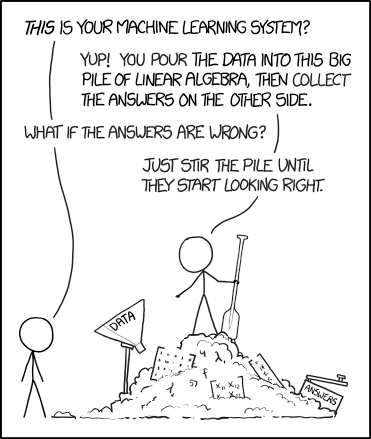
\includegraphics[height=0.55\textheight]{images/1838_machine_learning.png}
\end{center}
\bottomnote{XKCD \#1838 by Randall Munroe (CC BY-NC 2.5)}
\end{frame}

% SLIDE 3: Learning Objectives
\begin{frame}[t]{Learning Objectives}
\vspace{1em}
After this lecture, you will be able to:
\begin{itemize}
  \item \textbf{Interpret} KNN and K-Means visualizations to diagnose model behavior
  \item \textbf{Identify} when algorithms succeed and when they fail using diagnostic charts
  \item \textbf{Select} optimal hyperparameters ($k$, $n\_clusters$) using visual tools
\end{itemize}
\bottomnote{We cover 20 essential visualizations spanning KNN foundations, K-Means clustering, and advanced diagnostics}
\end{frame}

% SLIDE 4: Table of Contents
\begin{frame}{Outline}
  \tableofcontents
\bottomnote{Three parts: KNN Foundations, K-Means Clustering, Advanced Diagnostics}
\end{frame}

% ============================================================
% PART 1: KNN FOUNDATIONS (7 charts)
% ============================================================
\section{KNN Foundations}

% SLIDE 5: C1 --- KNN Decision Boundary
\begin{frame}[t]{How KNN Carves Up Feature Space}
\begin{center}

\includegraphics[width=0.65\textwidth]{01_knn_boundaries/chart.pdf}
\end{center}
\bottomnote{KNN creates flexible, non-linear boundaries that adapt to local data structure}
\end{frame}

% SLIDE 6: C2 --- Distance Metrics
\begin{frame}[t]{Distance Metrics: The Foundation of KNN}
\begin{center}

\includegraphics[width=0.65\textwidth]{02_distance_metrics/chart.pdf}
\end{center}
\bottomnote{The choice of distance metric fundamentally shapes which neighbors are ``nearest''}
\end{frame}

% SLIDE 7: C7 --- Feature Scaling
\begin{frame}[t]{Why Feature Scaling Is Non-Negotiable}
\begin{center}

\includegraphics[width=0.65\textwidth]{08_feature_scaling_effect/chart.pdf}
\end{center}
\bottomnote{Unscaled features with larger ranges dominate distance calculations}
\end{frame}

% SLIDE 8: C8 --- Bias-Variance
\begin{frame}[t]{The k Tradeoff: Bias vs Variance}
\begin{center}

\includegraphics[width=0.65\textwidth]{10_bias_variance_visual/chart.pdf}
\end{center}
\bottomnote{Small k = high variance (noisy), large k = high bias (over-smoothed)}
\end{frame}

% SLIDE 9: C9 --- CV Accuracy Curve
\begin{frame}[t]{Finding the Optimal k}
\begin{center}

\includegraphics[width=0.65\textwidth]{13_cv_accuracy_curve/chart.pdf}
\end{center}
\bottomnote{Cross-validation reveals the sweet spot between underfitting and overfitting}
\end{frame}

% SLIDE 10: A2 --- Curse of Dimensionality (NEW)
\begin{frame}[t]{The Curse of Dimensionality}
\begin{center}

\includegraphics[width=0.65\textwidth]{top10_12_curse_of_dimensionality/chart.pdf}
\end{center}
\bottomnote{As dimensions grow, all points become equidistant and KNN loses discriminative power}
\end{frame}

% SLIDE 11: A3 --- KNN Regression (NEW)
\begin{frame}[t]{KNN for Regression: Averaging Neighbors}
\begin{center}

\includegraphics[width=0.65\textwidth]{top10_13_knn_regression/chart.pdf}
\end{center}
\bottomnote{KNN regression averages neighbor values --- k controls the smoothness of predictions}
\end{frame}

% ============================================================
% TRANSITION
% ============================================================

% SLIDE 12: Transition
\begin{frame}[t]{From Supervised to Unsupervised}
\vspace{1.5em}
\begin{itemize}
  \item KNN needs labels --- it \textbf{classifies} based on neighbor votes
  \item K-Means discovers structure --- it \textbf{clusters} without labels
  \item Same distance intuition, fundamentally different tasks
\end{itemize}
\bottomnote{Both algorithms rely on distance, but KNN is supervised while K-Means is unsupervised}
\end{frame}

% ============================================================
% PART 2: K-MEANS FOUNDATIONS (6 charts)
% ============================================================
\section{K-Means Clustering}

% SLIDE 13: C3 --- K-Means Iterations
\begin{frame}[t]{K-Means: The Iterative Algorithm}
\begin{center}

\includegraphics[width=0.65\textwidth]{03_kmeans_iteration/chart.pdf}
\end{center}
\bottomnote{Each iteration alternates between assigning points and updating centroids}
\end{frame}

% SLIDE 14: C4 --- Elbow Method
\begin{frame}[t]{How Many Clusters? The Elbow Method}
\begin{center}

\includegraphics[width=0.65\textwidth]{04_elbow_method/chart.pdf}
\end{center}
\bottomnote{The ``elbow'' marks where adding clusters yields diminishing returns in inertia reduction}
\end{frame}

% SLIDE 15: C5 --- Silhouette
\begin{frame}[t]{Silhouette Analysis: Cluster Quality}
\begin{center}

\includegraphics[width=0.65\textwidth]{05_silhouette/chart.pdf}
\end{center}
\bottomnote{Silhouette scores measure how similar points are to their own cluster vs nearest neighbor cluster}
\end{frame}

% SLIDE 16: C6 --- Voronoi
\begin{frame}[t]{Voronoi Tessellation: K-Means Geometry}
\begin{center}

\includegraphics[width=0.65\textwidth]{06_voronoi/chart.pdf}
\end{center}
\bottomnote{K-Means partitions space into Voronoi cells --- each point belongs to its nearest centroid}
\end{frame}

% SLIDE 17: C10 --- Failure Cases (NEW, 1x2 subplot)
\begin{frame}[t]{When K-Means Fails: Cluster Shape Matters}
\begin{center}

\includegraphics[width=0.65\textwidth]{top10_10_kmeans_failure_cases/chart.pdf}
\end{center}
\bottomnote{K-Means assumes spherical clusters --- non-convex shapes require density-based methods}
\end{frame}

% SLIDE 18: A4 --- Init Sensitivity (NEW)
\begin{frame}[t]{Initialization Matters: Random vs K-Means++}
\begin{center}

\includegraphics[width=0.65\textwidth]{top10_14_kmeans_init_sensitivity/chart.pdf}
\end{center}
\bottomnote{K-Means++ provides smarter initialization, reducing sensitivity to starting positions}
\end{frame}

% ============================================================
% PART 3: ADVANCED DIAGNOSTICS (7 charts)
% ============================================================
\section{Advanced Diagnostics}

% SLIDE 19: A1 --- Weighted vs Uniform (NEW)
\begin{frame}[t]{Distance-Weighted KNN: Closer Neighbors Matter More}
\begin{center}

\includegraphics[width=0.65\textwidth]{top10_11_knn_weighted_vs_uniform/chart.pdf}
\end{center}
\bottomnote{Weighting by inverse distance reduces the influence of distant, possibly misleading neighbors}
\end{frame}

% SLIDE 20: A7 --- Gap Statistic (NEW)
\begin{frame}[t]{Gap Statistic: A Rigorous k Selection}
\begin{center}

\includegraphics[width=0.65\textwidth]{top10_17_gap_statistic/chart.pdf}
\end{center}
\bottomnote{The gap statistic compares clustering quality against a null reference distribution}
\end{frame}

% SLIDE 21: A9 --- Inertia Convergence (NEW)
\begin{frame}[t]{K-Means Convergence: Inertia per Iteration}
\begin{center}

\includegraphics[width=0.65\textwidth]{top10_19_kmeans_inertia_convergence/chart.pdf}
\end{center}
\bottomnote{K-Means typically converges within 10--15 iterations for moderate-sized datasets}
\end{frame}

% SLIDE 22: A5 --- Mini-Batch KMeans (NEW)
\begin{frame}[t]{Mini-Batch K-Means: Speed vs Quality}
\begin{center}

\includegraphics[width=0.65\textwidth]{top10_15_minibatch_kmeans/chart.pdf}
\end{center}
\bottomnote{Mini-batch updates trade marginal quality loss for dramatic speedup on large datasets}
\end{frame}

% SLIDE 23: A6 --- Cluster Centers Heatmap (NEW)
\begin{frame}[t]{Cluster Profiles: What Each Segment Looks Like}
\begin{center}

\includegraphics[width=0.65\textwidth]{top10_16_cluster_centers_heatmap/chart.pdf}
\end{center}
\bottomnote{Centroid feature values reveal the defining characteristics of each customer segment}
\end{frame}

% SLIDE 24: A8 --- KNN ROC Curves (NEW)
\begin{frame}[t]{KNN ROC Curves: Effect of k on Classification}
\begin{center}

\includegraphics[width=0.65\textwidth]{top10_18_knn_roc_curves/chart.pdf}
\end{center}
\bottomnote{Moderate k values typically achieve the best AUC by balancing precision and recall}
\end{frame}

% SLIDE 25: A10 --- KNN Confusion Matrix (NEW)
\begin{frame}[t]{KNN Confusion Matrix: Where Errors Happen}
\begin{center}

\includegraphics[width=0.65\textwidth]{top10_20_knn_confusion_matrix/chart.pdf}
\end{center}
\bottomnote{Confusion matrices reveal systematic misclassification patterns between classes}
\end{frame}

% ============================================================
% CLOSING
% ============================================================
\section{Summary}

% SLIDE 26: Summary Checklist
\begin{frame}[t]{20 Charts You Should Know}
\vspace{0.3em}
\begin{columns}[T]
\begin{column}{0.48\textwidth}
\footnotesize
\begin{enumerate}
  \item Decision Boundary
  \item Distance Metrics
  \item Feature Scaling
  \item Bias--Variance
  \item CV Accuracy
  \item Curse of Dimensionality
  \item KNN Regression
  \item Weighted vs Uniform
  \item KNN ROC
  \item KNN Confusion Matrix
\end{enumerate}
\end{column}
\begin{column}{0.48\textwidth}
\footnotesize
\begin{enumerate}
  \setcounter{enumi}{10}
  \item K-Means Iterations
  \item Elbow Method
  \item Silhouette
  \item Voronoi
  \item Failure Cases
  \item Init Sensitivity
  \item Gap Statistic
  \item Inertia Convergence
  \item Mini-Batch
  \item Cluster Profiles
\end{enumerate}
\end{column}
\end{columns}
\bottomnote{Master these 20 visualizations for KNN and K-Means mastery}
\end{frame}

% SLIDE 27: Closing XKCD
\begin{frame}[t]{And Remember\ldots}
\vspace{0.5em}
\begin{center}
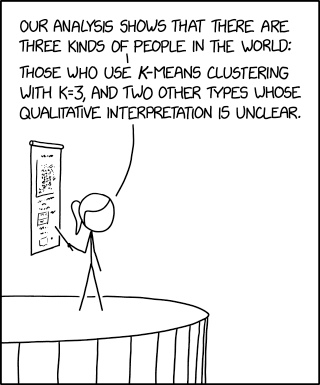
\includegraphics[height=0.55\textheight]{images/2731_kmeans_clustering.png}
\end{center}
\bottomnote{XKCD \#2731 by Randall Munroe (CC BY-NC 2.5)}
\end{frame}

\end{document}
